% written by Kei YASUDA 2017
% 応募要領指定フォントに準ずるために,xelatexを用いる。
\documentclass[base=10pt,magstyle=real,a4paper,twocolumn,xelatex,pandoc,jafont=noto]{bxjsarticle}%,jafont=ms
\usepackage{aij_johosympo_xelatex}

%font指定方法
%\mcfamily\mdseries,\textmc{\textmd{...}}:Noto Serif CJK Regular
%\mcfamily\bfseries,\textmc{\textbf{...}}:Noto Serif CJK Bold
%\sffamily\mdseries,\textsf{\textmd{...}}:Noto Sans CJK Regular
%\sffamily\bfseries,\textsf{\textbf{...}}:Noto Sans CJK Bold

\usepackage{hyperref}

%タイトル,著者,キーワードなどを記入
\title{情報システム利用技術に関する研究}
\subtitle{建築分野における情報システムの応用技術}
\foreigntitle{A Study on Computer Technology Symposium}
\foreignsubtitle{Application of information systems to architectural design and engineering}
\author{構造~一郎\textsuperscript{*1}
	   ,環境~二郎\textsuperscript{*1}
	   ,計画~三郎\textsuperscript{*2}
       }
\foreignauthor{Ichirou Kouzou\textsuperscript{*1}, 
			   Jirou Kankyo\textsuperscript{*1}, 
	           and Saburo Keikaku\textsuperscript{*2}
               }%英文での著者表記
\affiliation{
	\mbox{*1}&建築大学建築学科 教授 工博\\
			 &Professor, Department of Architecture, University of Kenchiku, Ph.D.\\
	\mbox{*2}&情報株式会社設計部 部長 博士(工学)\\
	         &Manager, Design Department, Joho Corporation, Ph.D.\\
}%アスタリスクは本文で打っても数式で打っても文字間などうまくいかない。
\ekeyword{Architecture; structure; environment; planning; information.}
\jkeyword{建築; 構造; 環境; 計画; 情報}

%%%---definition begin---%%%
\newcommand{\marker}[1]{\underline{\textbf #1}}

\usepackage{verbatim, setspace,framed}
\newcommand{\inputpython}[1]{
	\begin{oframed}
		\begin{spacing}{0.72}
			{\small 
				\texttt{\verbatiminput{#1}}
			}
		\end{spacing}
	\end{oframed}
}

%%%---definition end---%%%
\pagestyle{fancy}
%\thispagestyle{fancy}
\lhead{}
\chead{}
\rhead{}
\lfoot{論文 R00}
\cfoot{}
\rfoot{}


%ここから本文
\begin{document}

\begin{abstract}
	For long papers in Japanese, the summary should be written either in English. The maximum length of the summary is 200 words in English.
	Lorem ipsum dolor sit amet, consectetuer adipiscing elit. Aenean commodo ligula eget dolor. Aenean massa. Cum sociis natoque penatibus et magnis dis parturient montes, nascetur ridiculus mus. Donec quam felis, ultricies nec, pellentesque eu, pretium quis, sem. Nulla consequat massa quis enim. Donec pede justo, fringilla vel, aliquet nec, vulputate eget, arcu. In enim justo, rhoncus ut, imperdiet a, venenatis vitae, justo. Nullam dictum felis eu pede mollis pretium. Integer tincidunt. Cras dapibus. Vivamus elementum semper nisi. Aenean vulputate eleifend tellus. Aenean leo ligula, porttitor eu, consequat vitae, eleifend ac, enim. Aliquam lorem ante, dapibus in, viverra quis, feugiat a, tellus. Phasellus viverra nulla ut metus varius laoreet. Quisque rutrum. Aenean imperdiet. Etiam ultricies nisi vel augue. Curabitur ullamcorper ultricies nisi. Nam eget dui. Etiam rhoncus. Maecenas tempus, tellus eget condimentum rhoncus, sem quam semper libero, sit amet adipiscing sem neque sed ipsum. Nam quam nunc, blandit vel, luctus pulvinar, hendrerit id, lorem. Maecenas nec odio et ante tincidunt tempus. Donec vitae sapien ut libero venenatis faucibus. Nullam quis ante. Etiam sit amet orci eget
\end{abstract}
\maketitle %abstractの後にかいて,abstractを段組にしない
\thispagestyle{fancy}
\pagestyle{fancy}%draftの場合,ヘッダーを表示するとよい。
%\pagestyle{empty}%emptyにするとヘッダーは表示されない。
%\tableofcontents %目次


%\section{序論}
%	\subsection{背景}
%	\url{http://www.aij.or.jp/jpn/transaction/ronbun/}
%

\section{はじめに}
「論文」は6ページで構成する。

上下の余白は25mm,左右の余白は20mm。和文は明朝体,英文はローマン体を用いる。

タイトル,著者名,職位等,要旨,キーワードは1段組で,本文は2段組で記す。


\section{題目・著者名・所属等・英文要旨・キーワードについて}
\subsection{題目}
題目は日本語,英語の順で,14ポイント,ボールド,中央揃え(副題は10.5ポイント)。
英語題目主題はHeadline Capitalization,英語副題はSentence capitalizationとする。
\begin{itemize}
	\item Sentence capitalization: Symposium on computer technology of information, systems, and application 
	\item Headline capitalization: Symposium on Computer Technology of Information, Systems, and Application
\end{itemize}

\subsection{著者名}
著者名は日本語,英語の順に9~10ポイントの中央揃えで,日本語の発表者名に○印を付ける。*(合い印)は半角*を上付きにする。英語著者名はHeadline Capitalizationとする。

\subsection{所属等}
所属・職位・学位は日本語,英語の順に9~10ポイント,左揃えで記す
。日本語の所属等には半角の*と著者名に対応した番号を付ける。
英語の所属等はHeadline capitalization。

\subsection{英文要旨}
要旨は,本文が日本語の場合は9~10ポイントの英語で200words以内で記述する。

\subsection{キーワード}
キーワードは日本語,英語の順で,最大6つまでを9~10ポイントで中央揃え,それぞれをセミコロンで区切る。
英語のキーワードはSentence capitalizationとし,ピリオドで終わる。

題目と著者名の間,著者名と職位等の間,職位等と概要の間および概要とキーワードの間は1行あける。


\section{本文}
キーワードの下に2行あけて本文を記す。本文は2段組で,1段の幅は82mm,段組の間は6mmとし,1段にはなるべく25字×48行(文字の大きさ9ポイント相当)入るように設定する。
寸法内であれば,文字数で1文字,行数で1行程度の差があってもよい。
1ページ目については,題目等が入るので本文の行数は各自調整すること。本文の各段落の頭は,必ず字下げ(1文字)する。


\section{図表について}
\subsection{図について}
本文と図の間は1行空け,図は中央揃えにする。図幅は段の幅82mm以内または2段分の170mm以内。
図の次行には図番および図題を設け,図番および図題の下は1行空ける(\figref{fig:figuresympo})。
% TODO: \usepackage{graphicx} required
\begin{figure}[H]
	\centering
	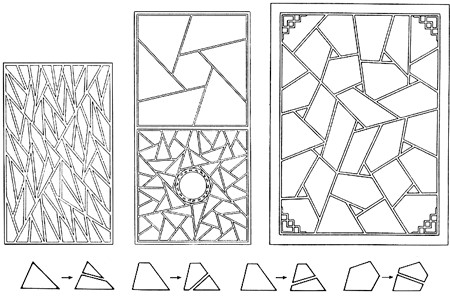
\includegraphics[width=1\linewidth]{../figure/figure_sympo.jpg}
	\caption{This is the caption of a figure. It goes below the figure}
	\label{fig:figuresympo}
\end{figure}

\subsection{表について}
本文との間に1行空け,表の前行に表番および表題を設ける。
表の幅は,段の幅82㎜以内または2段分の170mm以内とし,表の下は1行空ける(\tabref{tab:joho})。


\begin{table}[H]
	\caption{This is the caption of a table. It goes above the table.}
	\label{tab:joho}
	\fontsize{8pt}{10pt}\selectfont
	\centering
	\begin{tabular}{|p{36mm}|p{36mm}|}
		\hline 
		Please use Times New Roman font with a size of 8 points
		& Please use Times New Roman font with a size of 8 points
		\\ 
		\hline
		 & \\
		\hline
	\end{tabular} 
\end{table}


\section{参考文献}
6ページ目の最後には,区切り罫線の後に参考文献を8ポイント,行間11ポイントで記す
\footnote{注はこのように書く。あああああああああああああああああああ
ああああああああああああああああああああああああああああああああああ}。

\clearpage
\noindent
1234567890
1234567890
12345
\\2\\3\\4\\5\\6\\7\\8\\9\\10\\
1\\2\\3\\4\\5\\6\\7\\8\\9\\20\\
1\\2\\3\\4\\5\\6\\7\\8\\9\\30\\
1\\2\\3\\4\\5\\6\\7\\8\\9\\40\\
1\\2\\3\\4\\5\\6\\7\\48\\%
1234567890
1234567890
12345
\\2\\3\\4\\5\\6\\7\\8\\9\\10\\

\noindent \rule[0.5em]{\columnwidth}{0.5truept}\\
\begin{thebibliography}{9}
	\bibitem{参考文献1}
		8ポイント,行間11ポイントで記す。あああああ
        ああああああああああああああああああああああ
        あああああああああああああああああああああ
\end{thebibliography}
\vspace{1\Cvs}
%後注を出力
\theendnotes

\end{document}          
